%!TEX root = ../template.tex
%%%%%%%%%%%%%%%%%%%%%%%%%%%%%%%%%%%%%%%%%%%%%%%%%%%%%%%%%%%%%%%%%%%
%% chapter1.tex
%% NOVA thesis document file
%%
%% Chapter with introduction
%%%%%%%%%%%%%%%%%%%%%%%%%%%%%%%%%%%%%%%%%%%%%%%%%%%%%%%%%%%%%%%%%%%

\typeout{NT FILE chapter2.tex}%

\chapter{State of the Art}
\label{cha:State of the Art}

\prependtographicspath{{Chapters/Figures/Covers/}}

This chapter is divided into several sections. The first one gives an introduction to

\section{Identity Governance and Administration (IGA)}
\label{sec:IGA}

Identity Governance and Administration (IGA) plays a pivotal role in modern IT operations, enabling organizations to effectively manage user identities and access across the enterprise. It combines two critical components: Identity Governance and Identity Administration.

    Identity Governance focuses on:
        Visibility: Providing insights into user identities and access privileges.
        Segregation of Duties: Ensuring that conflicting roles are separated to prevent misuse.
        Role Management: Defining and assigning roles for efficient access control.
        Attestation: Regularly reviewing and validating access rights.
        Analytics and Reporting: Leveraging data for informed decision-making.

    Identity Administration encompasses:
        Account Administration: Managing user accounts and their attributes.
        Credentials Administration: Handling passwords, tokens, and other authentication factors.
        User and Device Provisioning: Automating user access throughout their lifecycle.
        Managing Entitlements: Controlling permissions and authorizations.


\subsection{Definition and Purpose}
\label{sec:Template}

Explain what IGA is: Identity Governance and Administration (IGA) is a set of policies and practices that enable organizations to manage and secure digital identities for users, applications, and data. Highlight its purpose: IGA helps balance the need to provide automated access to technology assets while managing security and compliance risks

\subsection{Components of IGA}
\label{sec:Template}

Identity Lifecycle Management: Covers user provisioning, deprovisioning, and modification of access rights throughout an individual’s lifecycle within an organization. Access Governance: Focuses on defining and enforcing policies related to access control, segregation of duties, and entitlement management. Access Administration: Involves managing user access requests, approvals, and access reviews. Role-Based Access Control (RBAC): Describes how roles are defined and assigned to users based on their job responsibilities. Policy Enforcement and Compliance: Ensures adherence to security policies, regulations (such as SOX, HIPAA, and GDPR), and audit requirements.

\subsection{Challenges and Considerations}
\label{sec:Template}

Complexity: IGA implementations can be intricate due to diverse user populations, applications, and data sources. Integration: Integrating IGA with existing systems and applications can be challenging. Scalability: As organizations grow, scalability becomes crucial. User Experience: Balancing security with a positive user experience is essential.

\section{Netwrix Usercube}
\label{sec:Template}

Netwrix Usercube is a product that is now part of Netwrix. It is a comprehensive identity and access management solution. Netwrix Usercube enables organizations of all sizes to enhance their security and compliance posture by ensuring that access permissions are granted only to those who need them. It can automate onboarding and offboarding processes, easing the compliance burden.

The application is better described dividing it in two modules that work together: Identity Management and Hab

\subsection{Identity Management}
\label{sec:Template}

A company involves many sorts of identities: obviously employees, but also external workers like contractors who are usually not tracked in the company's systems except for billing purposes, bots, softwares, etc. All identity types that need to be assigned entitlements to work within the company must be represented.

Companies often use about one system for each identity type. Usercube capitalizes on information from several source systems in order to build a central repository meant to contain all the data necessary to manage all identities throughout their whole lifecycle.

Usercube's central repository acts as an intermediary between the systems that provide data, for example the HR system, and those that receive data, for example the Active Directory. This greatly reduces the complexity in the links between all systems.

Without an intermediary, adding one system to a set of n systems requires up to n sets of rules, one for each reading/writing relationship that this system has with the others. The complexity is quadratic.

Now with the central repository as an intermediary, implementing a new system requires only one more set of rules. The complexity becomes linear \cite{UsercubeDocument}.

\begin{figure}[htbp]
  \centering
  \begin{minipage}{0.48\textwidth}
    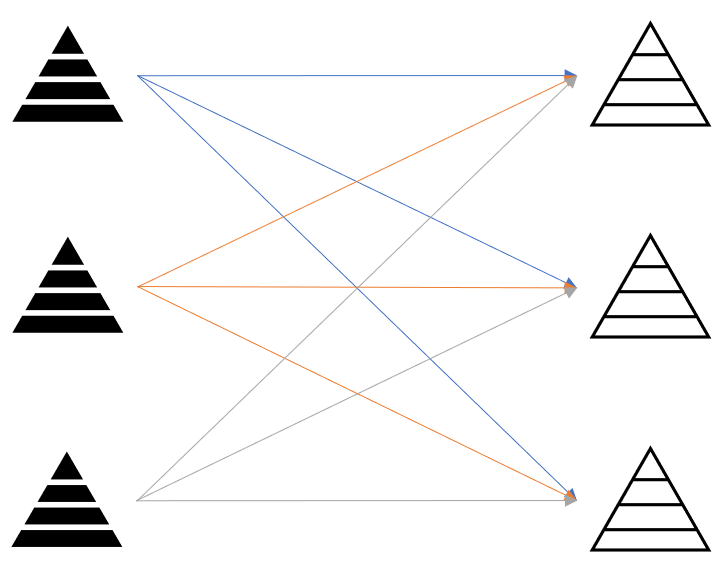
\includegraphics[width=\linewidth]{Identities_complexityQuadratic}
    \caption{Quadratic Complexity}
    \label{fig:Identities_complexityQuadratic}
  \end{minipage}\hfill
  \begin{minipage}{0.48\textwidth}
    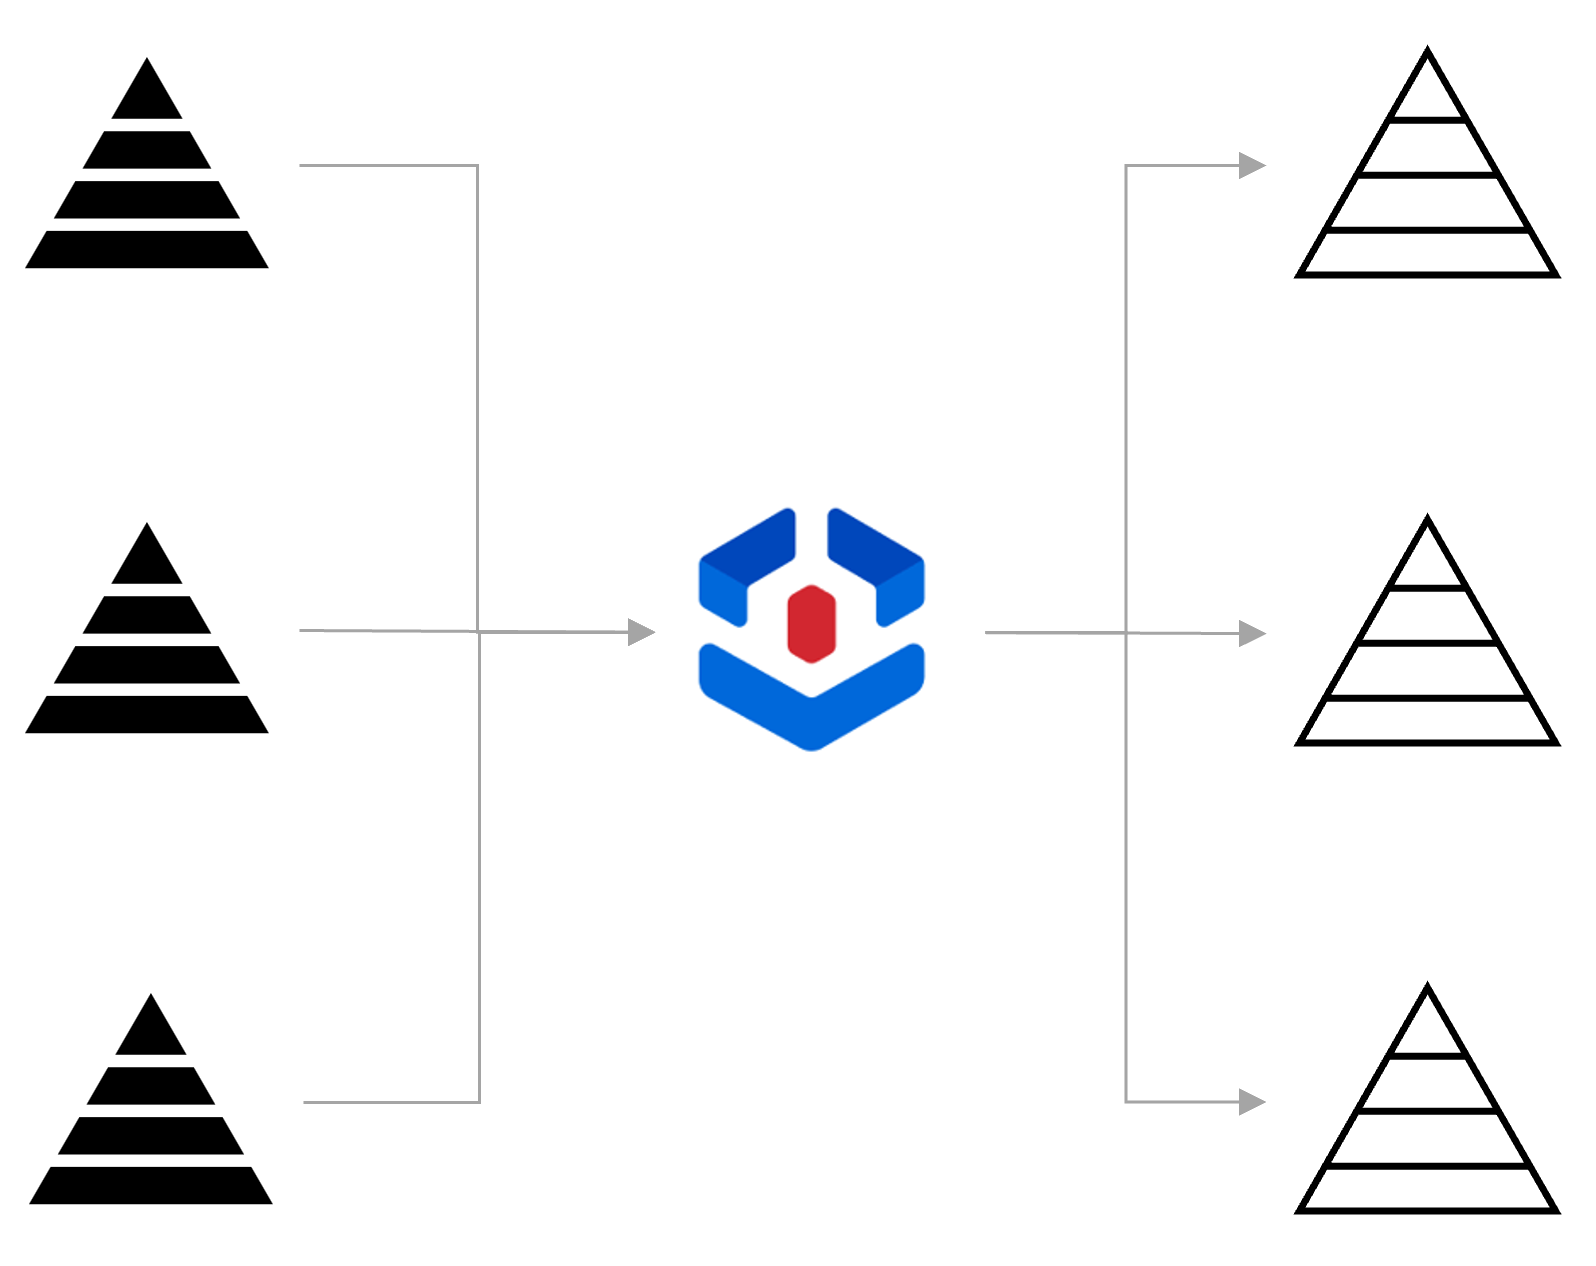
\includegraphics[width=\linewidth]{Identities_complexityLinear}
    \caption{Linear Complexity}
    \label{fig:Identities_complexityLinear}
  \end{minipage}
\end{figure}


\subsection{Entitlement Management}
\label{sec:Template}

Managing identities' entitlements requires managing entitlements and assigning them to identities. This page is about the role model.

Role Model Overview
A managed system's entitlements can have many forms. They authorize identities to access certain data on a given system, or a physical location.

For example, entitlements in the Active Directory are usually group memberships. For example, to have administrator rights in the Iris application, a user must be part of the members of the group SGAPPIT/Development/Iris/Administrator.

Usercube is designed to help establish an exhaustive and reliable catalog of the entitlements available in the managed systems, and assign the right entitlements to the right users.

Thus, the role model contains:

the entitlements, as roles, for all managed systems;
the rules that trigger the assignment of entitlements to identities, and more broadly manage the systems' resources. Some of them act as link between Usercube's roles and the systems' accounts and permissions. Some of them are linked to, and thus apply only to, specific resource types.

\begin{figure}[htbp]
  \centering
  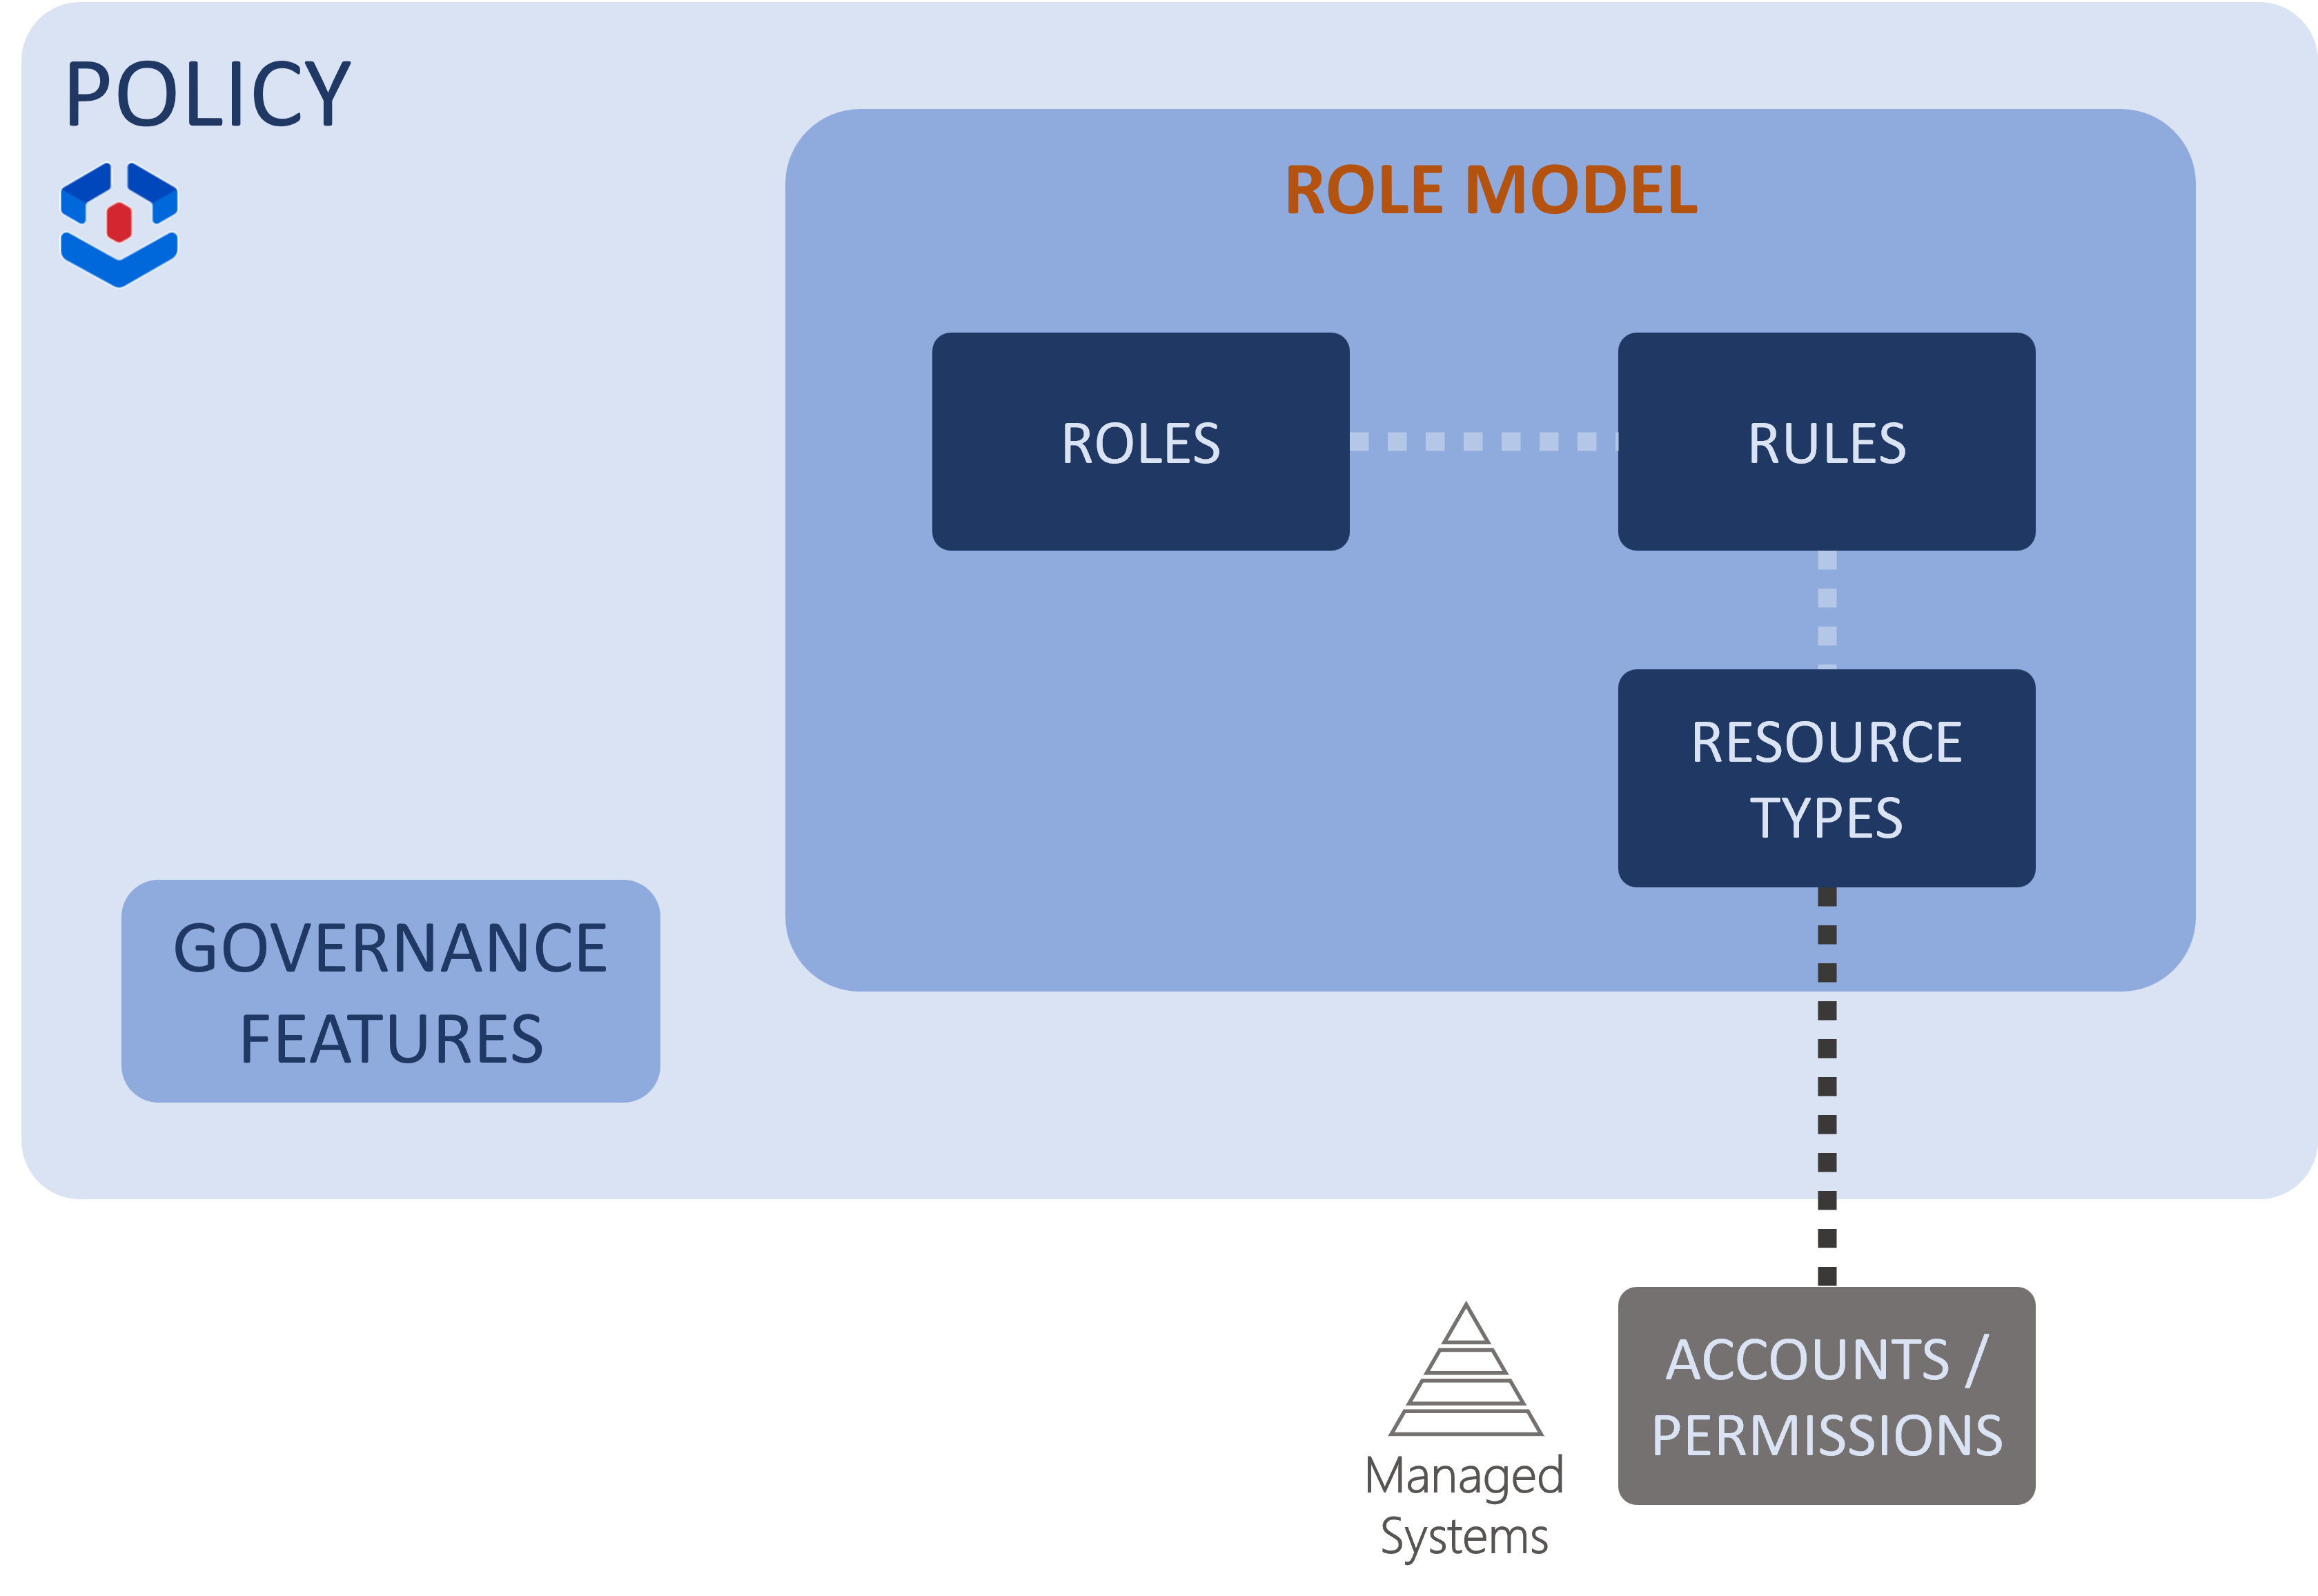
\includegraphics[width=5in]{Entitlements_RoleModel}
  \caption{Entitlements Role Model}
  \label{fig:configurationCycle}
\end{figure}

The role model is a subset of a policy that also includes governance data such as risk definition. So, at a higher level, distinct policies can be used to implement distinct behaviors.

A Role Catalog
Usercube intends to represent IGA-related access right mechanisms by a role-based model. The goal of the role catalog is contain an exhaustive list of entitlements from all managed systems.

Entitlements from the managed systems are modeled by roles. For each entitlement, NETWRIX advises creating a single role, with an easily understandable name, more functional than technical, so that everyone knows what the role is for.

Each individual entitlement should usually be modeled by a single role, and single roles can be grouped together into composite roles to be closer to real job positions.

A Rule Set
Roles alone are not enough to give identities the systems' technical entitlements. We need rules to have Usercube write users' entitlements in the managed systems. Rules are further used to automatically assign roles to users, or to categorize users and accounts, etc.

Provisioning rules
Just like identities, accounts are represented in Usercube by an entity-relationship model. So Usercube manages entitlements as resources' attribute values.

For example, giving specific Active Directory permissions to a new user means not only creating a new AD account, but also setting values for certain account properties like cn, sAMaccountName, userAccountControl or dn, etc.

Provisioning rules write the actual entitlements to the managed systems, most often based on users' roles.

For example, to give an AD entitlement to a user, we usually need to give them a group membership. Thus, we should have a rule that, when a user is assigned a specific role, adds the user to the member list of a specific AD group.

Even when a role is manually assigned, provisioning rules will determine which account (and permission groups) are given as entitlements.

Usercube's provisioning rules are:

- scalar rules to compute simple string properties;
- navigation rules and query rules to compute properties that act as foreign keys in a database;
- resource type rules to automatically create resources.

Assignment rules
While the role catalog and provisioning rules are together enough to manually give users their access rights, we often want Usercube to do this automatically. Assignment rules automatically assign roles to identities based on specific criteria.

For example, we can choose to assign the role Benefits Manager - FR to any user whose job title is benefits manager and whose location is in France.

Once all assignment rules are created, Usercube is able to spot existing assignments that are not supported by any rule, marking them as non-conforming. See more details on governance.

Usercube's assignment rules are:

- single role rules and composite role rules to assign single and composite roles;
- resource type rules to assign accounts.

Categorization rules
Different resources can be managed through different rules, by being part of different resource types. So a resource type is a group a resources that have the same IGA-related purposes. Categorization rules categorize resources into resource types and link identities to the accounts they own.

For example, we might need to differentiate AD's standard accounts from administration accounts. This way, we can configure different email addresses for privileged accounts, for example adm.john.smith@contoso.com. We can also add more approval steps in the workflows related to privileged accounts, for more security than for standard accounts.

\subsection{Architecture}
\label{sec:Template}

Usercube works via a server which operates computation, stores all application data in the database, and serves a web User Interface; at least one agent which operates data flows to/from the managed systems. The managed systems' credentials are used only by the agent and are never disclosed to the server. The agent can call the server, but the server cannot call the agent. The data flows' initiatives are always from the agent. In our case the installation is on-premises so that the server is installed on an isolated network within the company.

\begin{figure}[htbp]
  \centering
  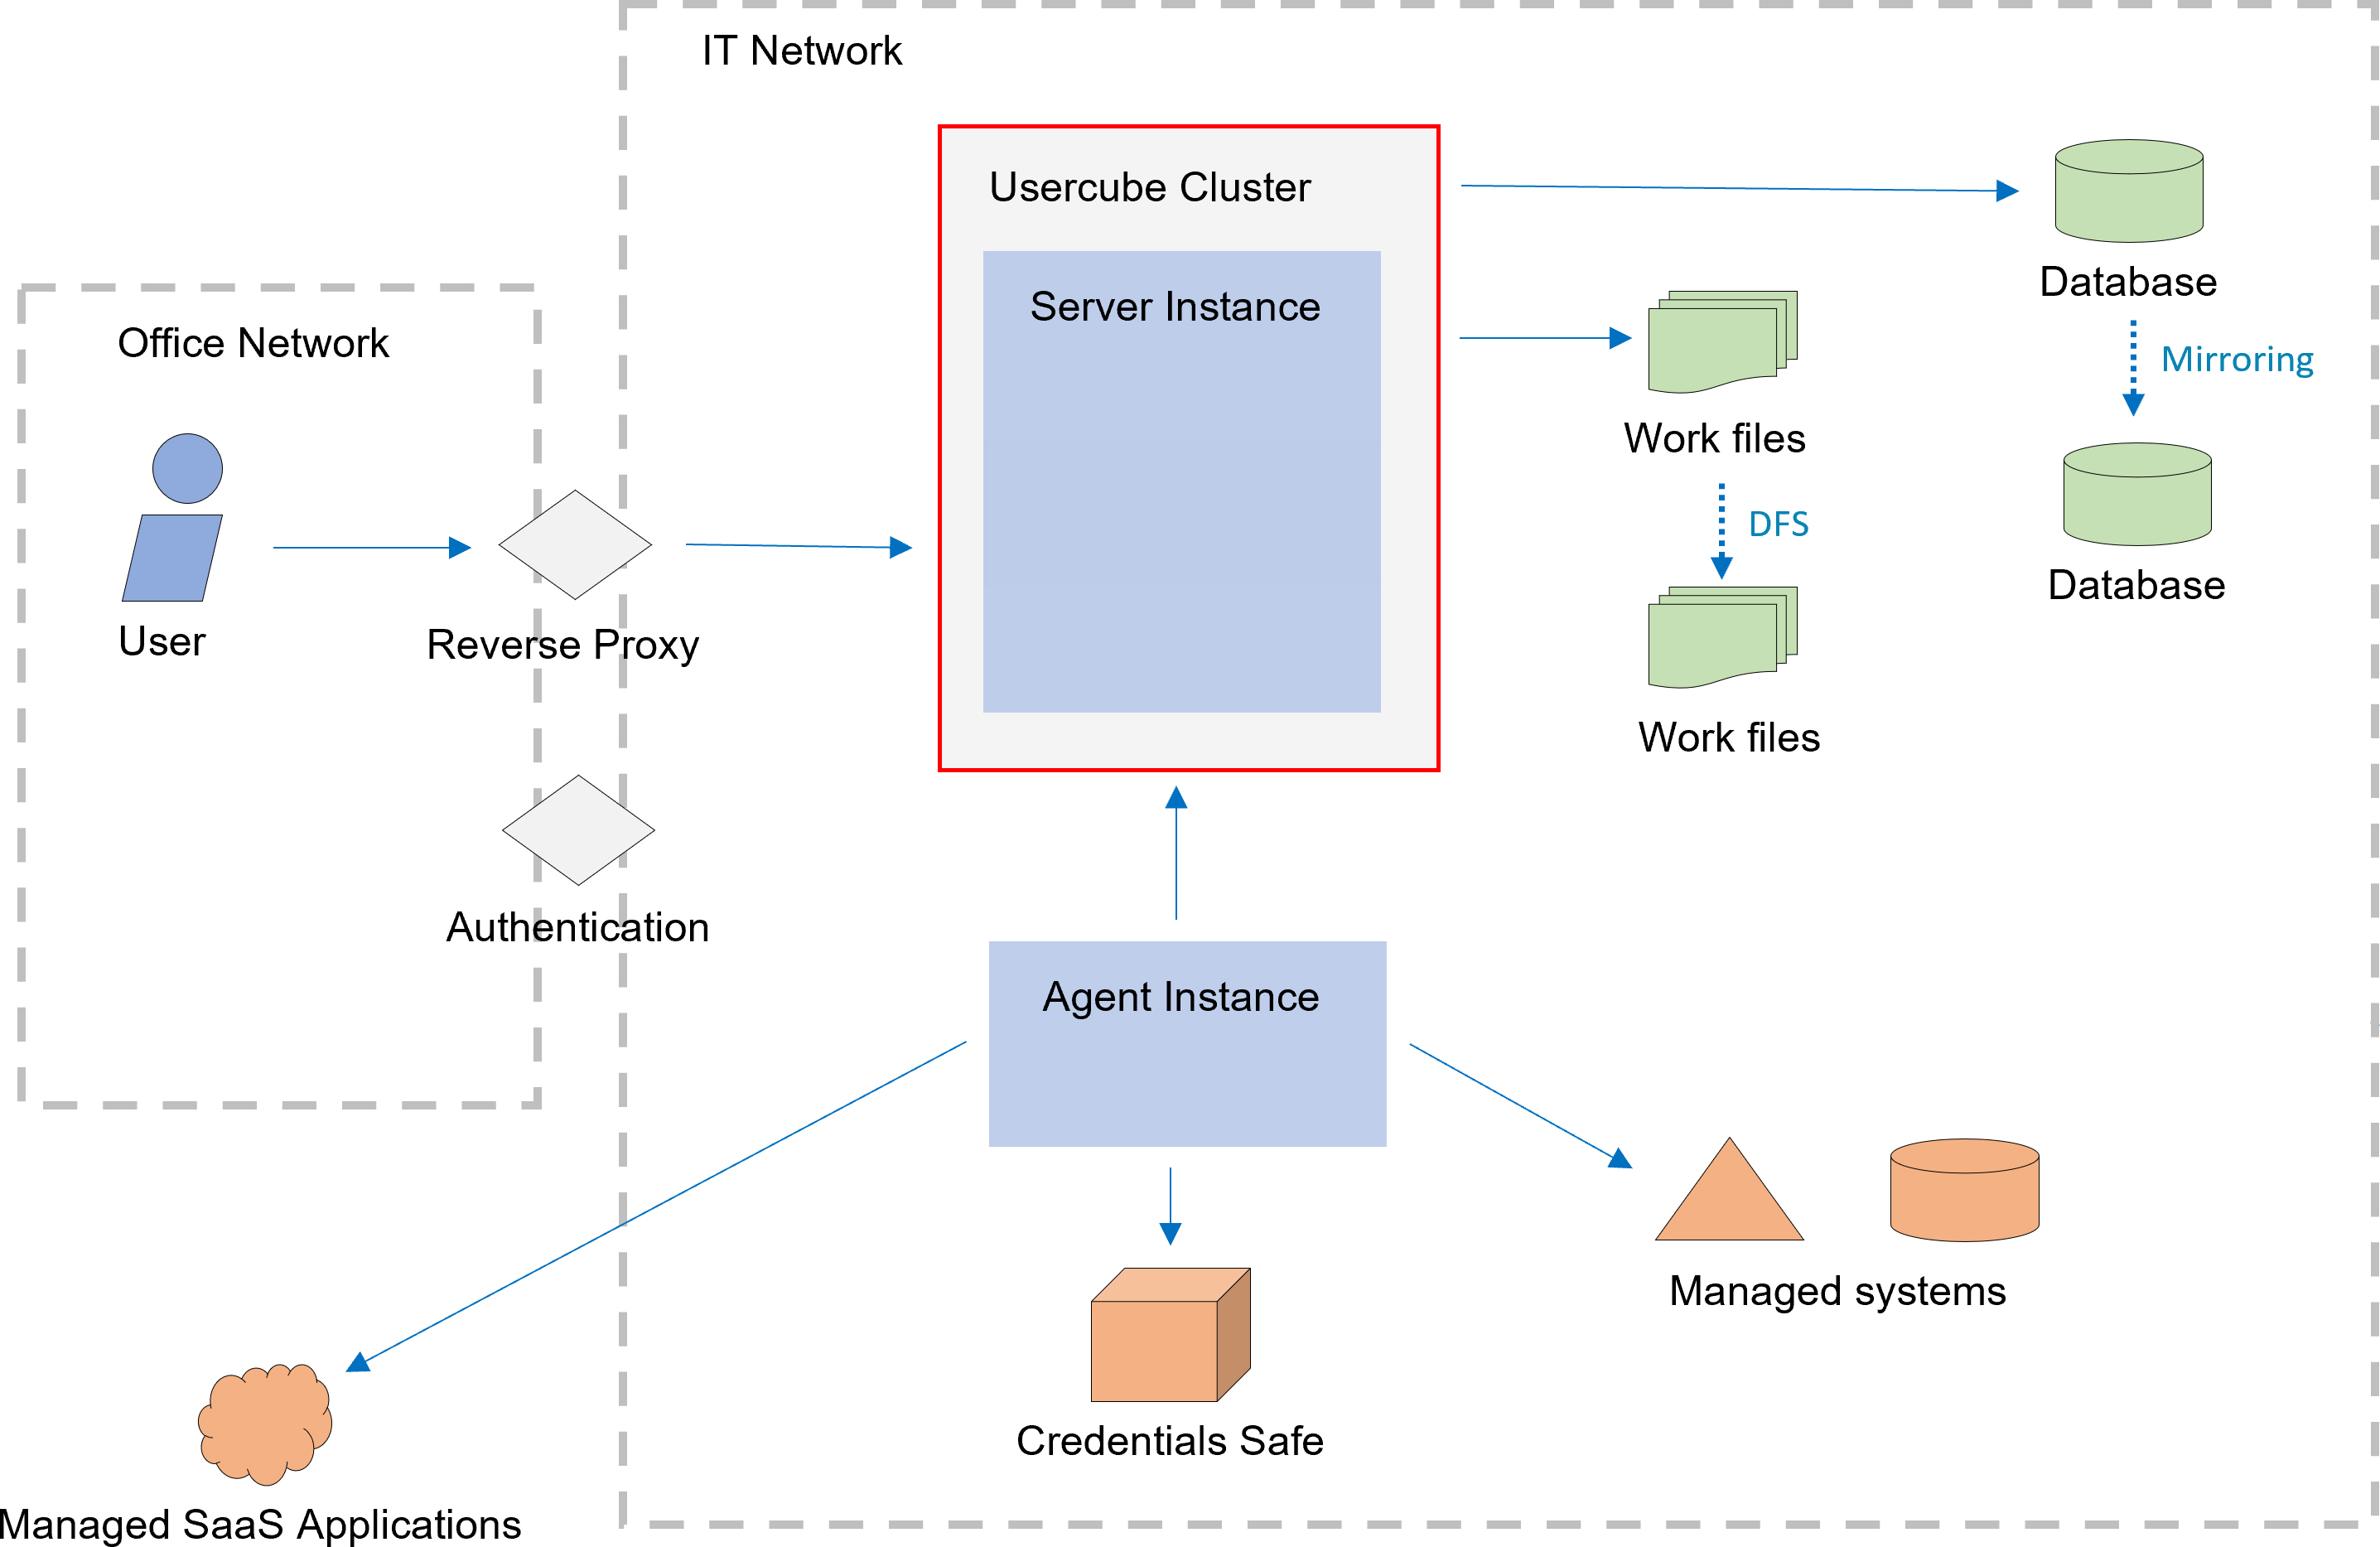
\includegraphics[width=5in]{Architecture_onPrem}
  \caption{Architecture on premises}
  \label{fig:Architecture_onPrem}
\end{figure}

\subsection{Configuration}
\label{sec:Template}

A Usercube configuration is a set of XML files edited according the Usercube schema. The recommendations part of this section explains how to set up an editing environment for the configuration. Regardless of the editing space, the configuration persists in the Usercube database. It's this stored configuration that is used at runtime. The Deploy configuration tool is used to import a new version of the configuration (from the XML files set). The Export configuration tool can be used to export the current configuration (to a XML files set). The Usercube project's integration cycle consists in developing a configuration by successive imports in a test instance.

The XML configuration schema shows some similarities with the database schema but they are not the same.

\begin{figure}[htbp]
  \centering
  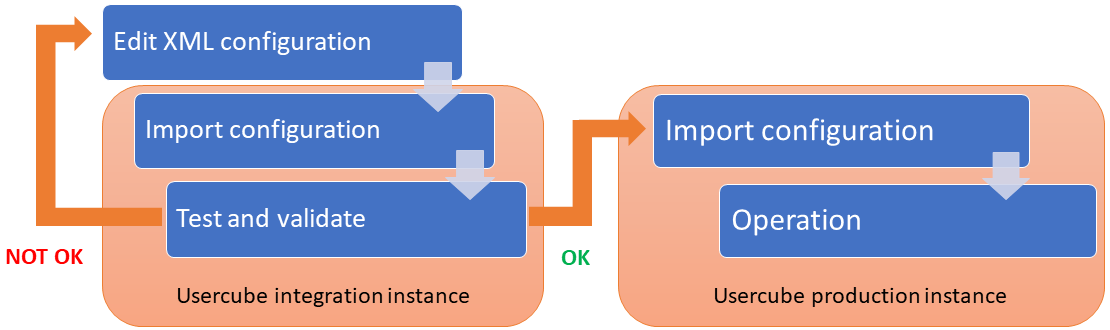
\includegraphics[width=5in]{configurationCycle}
  \caption{Usercube's configuration Cycle}
  \label{fig:configurationCycle}
\end{figure}

\subsection{Testing}
\label{sec:Template}

for testing we have different enviroments running in virtual machines. we deploy the new configuration to a testing instance and check if there is initial erros. Then the functional team is the one responsible to test the developments. After the test is done they send us back the ticket and then we save our code to build the next mep

\subsection{Deployment}
\label{sec:Template}

Deploy a local XML configuration by using the Deploy-Configuration executable and declaring at least: the configuration directory; the connection string of the database.

\section{Software Quality}
\label{sec:Template}

\subsection{Reverse Engineering}
\label{sec:Development models}

Reverse Engineering Involves analysing a subject system to determine its components and relationship between them Involves creation of alternative representations of the system, usually at a higher level of abstraction Does not involve changing or replicating system Only concerned with an examination of the system Can occur at any stage in s/w develop. life cycle

\subsection{Development models}
\label{sec:Development models}

\subsection{Lehman’s laws of software evolution}
\label{sec:Lehman}

The Lehman Laws of S/w evolution and S/w development process models address different aspects of the software development life cycle. However, they are related in the sense that both provide insights into the challenges and dynamics of software development over time S/w development process models define ways in which S/w projects are planned, executed, and controlled The Lehman Laws: Describe the evolution of S/w Suggest that S/w must continually evolve to remain useful.

\subsection{Refactoring}
\label{sec:Refactoring}

\cite{fowler2018refactoring}
Martin Fowler [Fow99]: "a disciplined technique for restructuring an existing body of code, altering its internal structure without changing its external behaviour." William Wake [Wak04]: "Refactoring is the art of improving the design of existing code. Refactoring provides us with ways to recognize problematic code and gives us recipes for improving it."


\section{Related Work}
\label{sec:Template}